% Created 2022-11-24 Thu 10:18
\documentclass[9pt, b5paper]{article}
\usepackage{xeCJK}
\usepackage{minted}
\usepackage[T1]{fontenc}
\usepackage[scaled]{beraserif}
\usepackage[scaled]{berasans}
\usepackage[scaled]{beramono}
\usepackage{graphicx}
\usepackage{xcolor}
\usepackage{multirow}
\usepackage{multicol}
\usepackage{float}
\usepackage{textcomp}
\usepackage{algorithm}
\usepackage{algorithmic}
\usepackage{latexsym}
\usepackage{natbib}
\usepackage{geometry}
\geometry{left=1.2cm,right=1.2cm,top=1.5cm,bottom=1.2cm}
\newminted{common-lisp}{fontsize=\footnotesize} 
\usepackage[xetex,colorlinks=true,CJKbookmarks=true,linkcolor=blue,urlcolor=blue,menucolor=blue]{hyperref}
\author{deepwaterooo}
\date{\today}
\title{Unity Export 导出到Android Studio再打包大致过程}
\hypersetup{
  pdfkeywords={},
  pdfsubject={},
  pdfcreator={Emacs 27.2 (Org mode 8.2.7c)}}
\begin{document}

\maketitle
\tableofcontents


\section{导出的unity项目文件大致是这样的}
\label{sec-1}
\begin{itemize}
\item 大致过程记一下,用作参考,原理还没有吃透,细节又比较多,容易忘记.作个笔记记一下,给自己用作参考
\end{itemize}

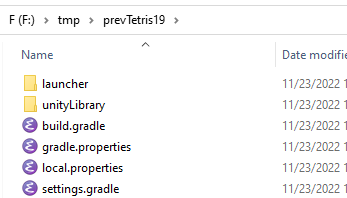
\includegraphics[width=.9\linewidth]{./pic/unityToAndroid_20221123_222322.png}
\begin{itemize}
\item 下面是2019年的版本可以打出两个文件夹,一个主工程,一个类库的导出包,2017年我用的版本打不出来,还需要想得再深一点多点儿,到可以按照这个笔记过程打包才行
\end{itemize}
\section{Android创建、unity导入}
\label{sec-2}
\subsection{首先新建一个Android项目}
\label{sec-2-1}

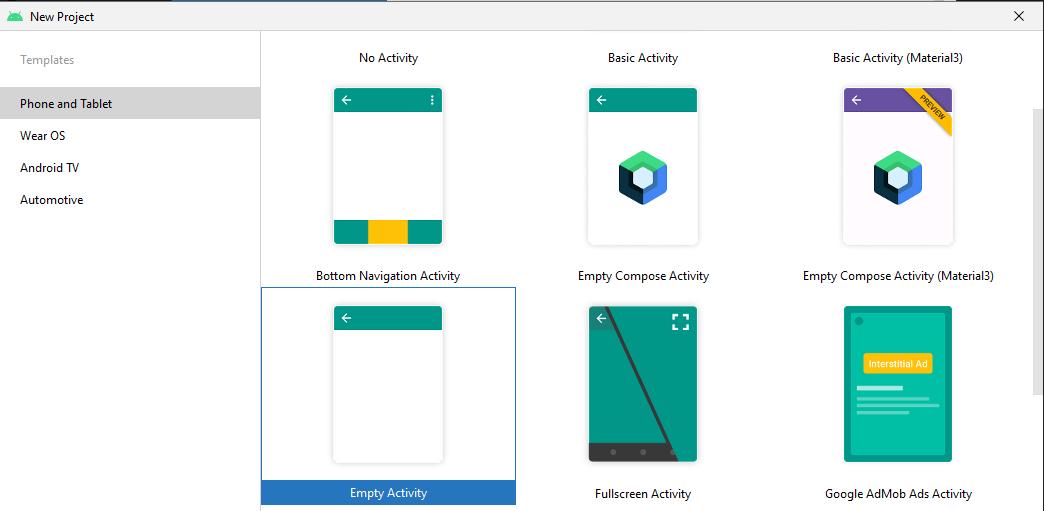
\includegraphics[width=.9\linewidth]{./pic/unityToAndroid_20221123_222542.png}
\begin{itemize}
\item 包名Package name跟unity的包名设置成一致,unity包名一般是 \textbf{com.unity3d.player} 。包名不一致的话,我试过也可以实现,但是在调用的时候要指明包,容易混淆,可能还有其他的一些问题,个人也不是很清楚。推荐保持一致,避免麻烦。Android项目名Name等随意。
\end{itemize}
\subsection{将unity项目以Module的方式导入Android}
\label{sec-2-2}

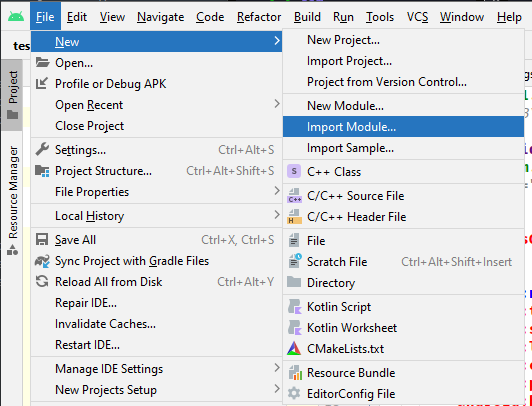
\includegraphics[width=.9\linewidth]{./pic/unityToAndroid_20221123_222637.png}

\subsection{选择unityLibrary导入。点击Finish}
\label{sec-2-3}

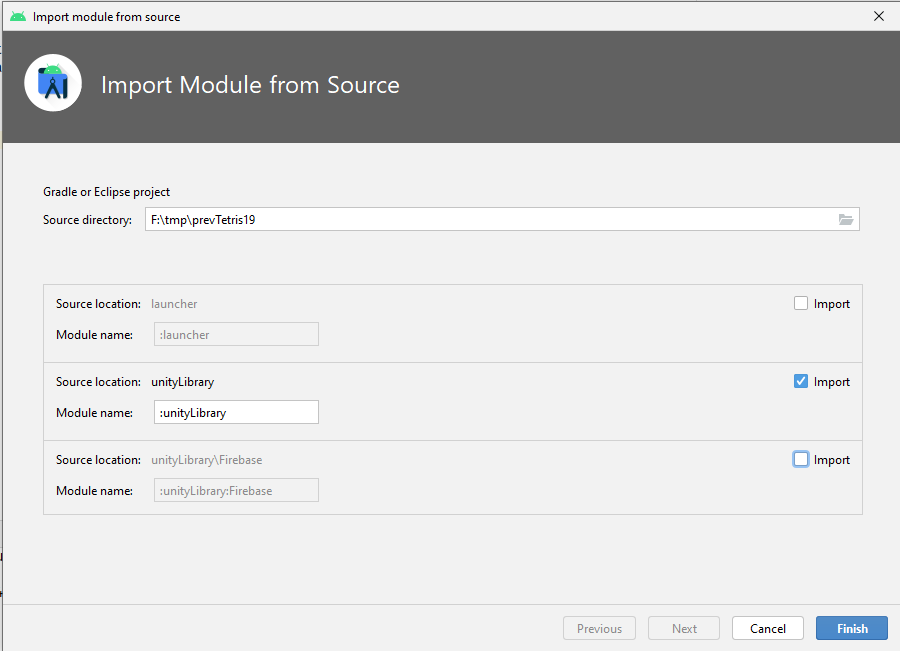
\includegraphics[width=.9\linewidth]{./pic/unityToAndroid_20221123_222720.png}
\subsection{导入之后,为Android添加unityLibrary的引用}
\label{sec-2-4}
\begin{itemize}
\item 左上角File——>Project Structure\ldots{}
\item 选择Dependencies  ——>  app ,然后点击右边这个加号 + ,选择第三个Moudule Dependency
\end{itemize}

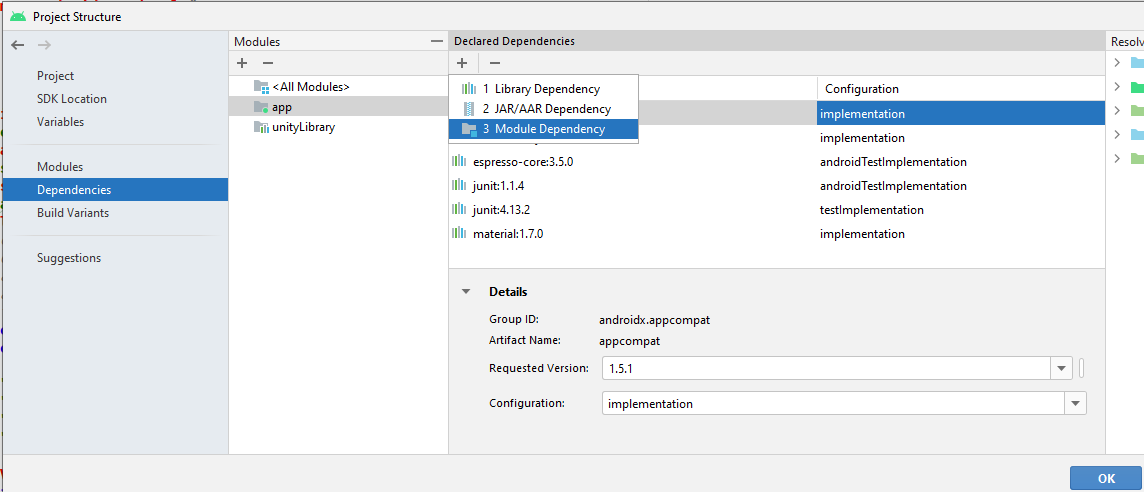
\includegraphics[width=.9\linewidth]{./pic/unityToAndroid_20221123_220755.png}
\begin{itemize}
\item 勾选刚刚导入的unity,点击OK。再点击上图的OK。
\end{itemize}

\subsection{配置 Android 以及 unity 的 build.gradle 文件}
\label{sec-2-5}
\begin{itemize}
\item 将SDK配置成当前Android版本可以运行。Android 以及unity的SDK确保要一样,不然会报错,比如这个minsdk。Build无误就算是导入完成了!

\item 这里作些简单的版本修改适配自己的手机,到项目可以构建成功为止.
\end{itemize}

\section{Android  启动运行 unity}
\label{sec-3}
\subsection{在unity的AndroidMainfest.xml文件}
\label{sec-3-1}
\begin{itemize}
\item 把<intent-filter>-->删掉或者注释掉,留着的话,当我们把程序运行到手机或者模拟机上时会有两个图标。
\item 其次是在<activity>里加入这行代码,实现多线程,避免在从unity返回Android时也将Android界面也结束了。
\begin{minted}[fontsize=\scriptsize,linenos=false]{xml}
android:process=":raadidcard"
\end{minted}
\end{itemize}

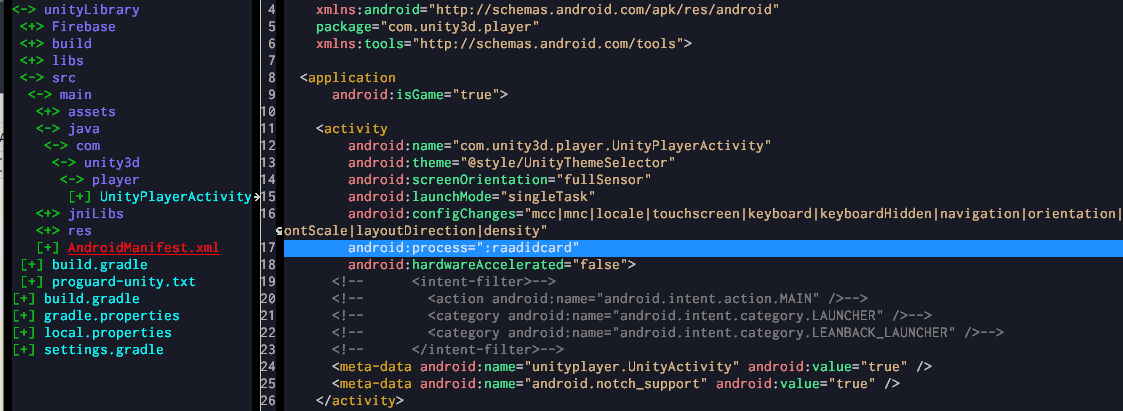
\includegraphics[width=.9\linewidth]{./pic/unityToAndroid_20221123_223227.png}
\subsection{在app的AndroidMainfest.xml文件里,在图中位置加入这两行代码:}
\label{sec-3-2}
\begin{minted}[fontsize=\scriptsize,linenos=false]{xml}
xmlns:tools="http://schemas.android.com/tools"

tools:replace="android:icon,android:theme,android:allowBackup"
\end{minted}
\begin{itemize}
\item 可以成片复制的代码如下:
\begin{minted}[fontsize=\scriptsize,linenos=false]{xml}
<?xml version="1.0" encoding="utf-8"?>
<manifest xmlns:android="http://schemas.android.com/apk/res/android"
          xmlns:tools="http://schemas.android.com/tools"
          package="com.unity3d.player">

  <application
      android:allowBackup="true"
      android:dataExtractionRules="@xml/data_extraction_rules"
      android:fullBackupContent="@xml/backup_rules"
      android:icon="@mipmap/ic_launcher"
      android:label="@string/app_name"
      android:roundIcon="@mipmap/ic_launcher_round"
      android:supportsRtl="true"
      tools:replace="android:icon,android:theme,android:allowBackup"
      android:theme="@style/Theme.Test"
      tools:targetApi="31">

    <activity
        android:name=".MainActivity"
        android:exported="true">
      <intent-filter>
        <action android:name="android.intent.action.MAIN" />
        <category android:name="android.intent.category.LAUNCHER" />
      </intent-filter>
      <meta-data
          android:name="android.app.lib_name"
          android:value="" />
    </activity>

  </application>
</manifest>
\end{minted}
\end{itemize}

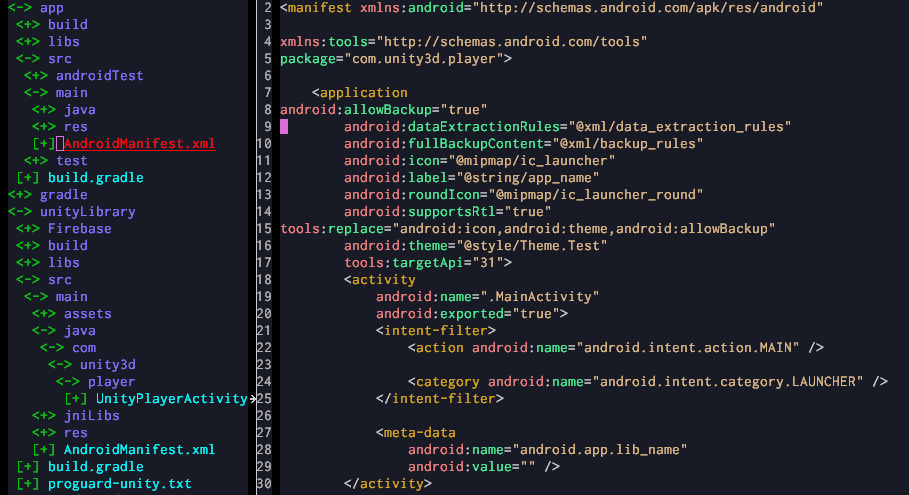
\includegraphics[width=.9\linewidth]{./pic/unityToAndroid_20221123_223757.png}

\subsection{在app的build.gradle里加入这行代码。}
\label{sec-3-3}
\begin{minted}[fontsize=\scriptsize,linenos=false]{xml}
ndk {
    abiFilters 'armeabi-v7a'
}
\end{minted}

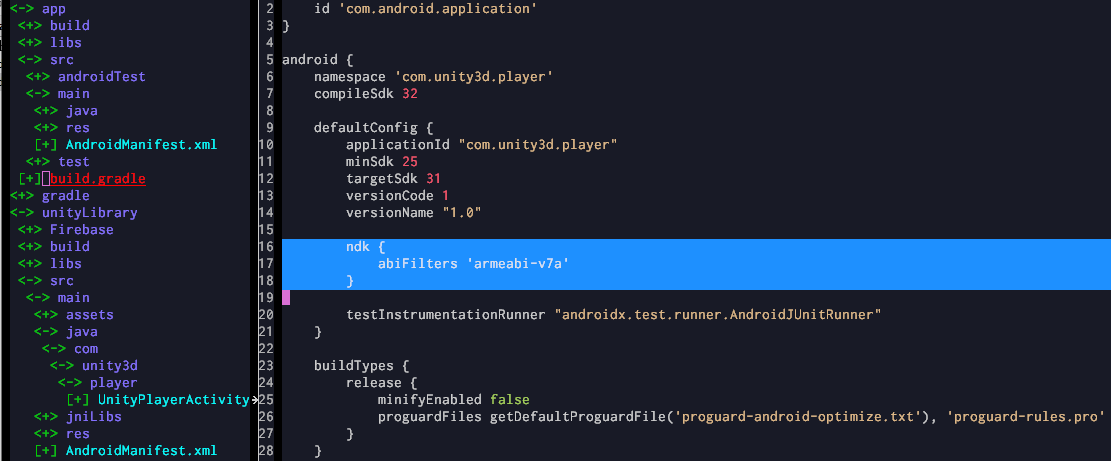
\includegraphics[width=.9\linewidth]{./pic/unityToAndroid_20221123_223842.png}
\subsection{在app的main->res->values->strings.xml里加入这行代码}
\label{sec-3-4}
\begin{itemize}
\item 都还没有去想,这句话能起到什么作用,应该是关系不大,或是可以跳过绕过的小细节
\begin{minted}[fontsize=\scriptsize,linenos=false]{xml}
<string name="game_view_content_description">Game view</string>
\end{minted}
\item 进行这两步操作的原因是,我在运行到手机时,他显示硬件不支持或者闪退。加入上面两个代码后就可以正常启动unity。
\item 我个人认为真正起作用的是上上一步关于手机架构的设置的ndk那三行,与上面字符串无关,应该是无关的
\end{itemize}

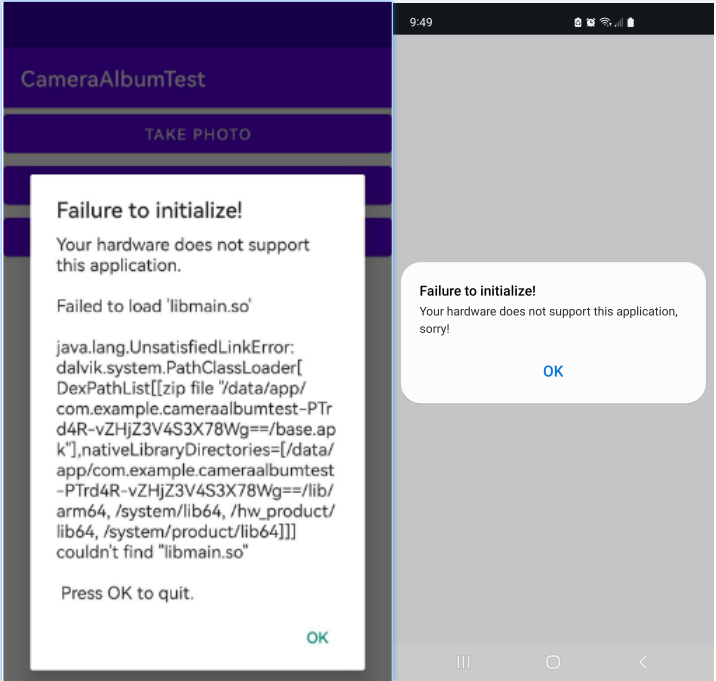
\includegraphics[width=.9\linewidth]{./pic/unityToAndroid_20221123_225409.png}

\subsection{点击按钮启动unity(画蛇添足)}
\label{sec-3-5}
\begin{itemize}
\item 感觉这个连接过程对于自己的项目就是画蛇添足.可是如何既能避开这一步,又能两者很好的平滑交互呢? 对于现在的自己,是个问题和挑战
\item 在主工程的activity\_main.xml 文件里添加一个按钮。MainActivity.java 里加入启动事件,如果在这里layout标红的话,就把鼠标移到layout下面,建立一个layout就行,我分析是主工程的问题,这个影响不大
\end{itemize}
\begin{minted}[fontsize=\scriptsize,linenos=false]{xml}
<Button
    android:id="@+id/showUnityBtn"
    android:layout_width="match_parent"
    android:layout_height="wrap_content"
    android:text="Show Unity"/>
\end{minted}

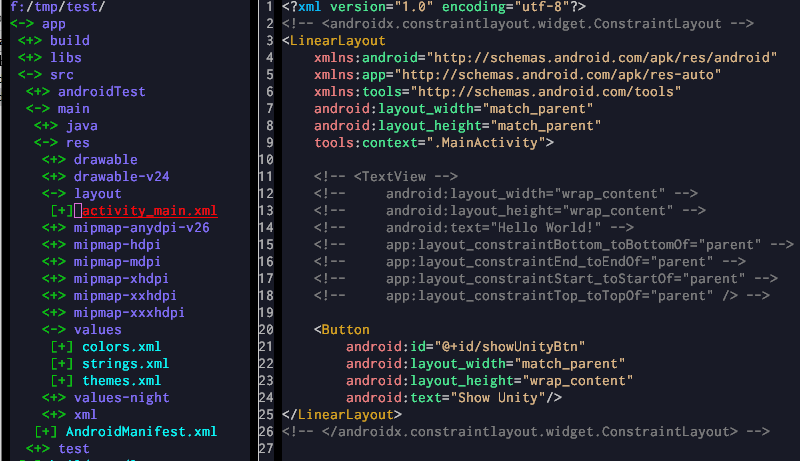
\includegraphics[width=.9\linewidth]{./pic/unityToAndroid_20221123_223751.png}
\begin{itemize}
\item MainActivity.cs 里的回调设置
\end{itemize}
\begin{minted}[fontsize=\scriptsize,linenos=false]{java}
Button btn = (Button)findViewById(R.id.showUnityBtn);
btn.setOnClickListener(new View.OnClickListener() {
        @Override
        public void onClick(View view) {

// <<<<<<<<<<<<<<<<<<<< UnityPlayerActivity <= com.unity3d.player 这里就是刚刚那个包名奇怪的地方,要不然 找不到 下面的 UnityPlayerActivity 类
            Intent intent = new Intent(MainActivity.this, UnityPlayerActivity.class); // <<<<<<<<<<<<<<<<<<<< UnityPlayerActivity

            startActivity(intent);
        }
    });
\end{minted}

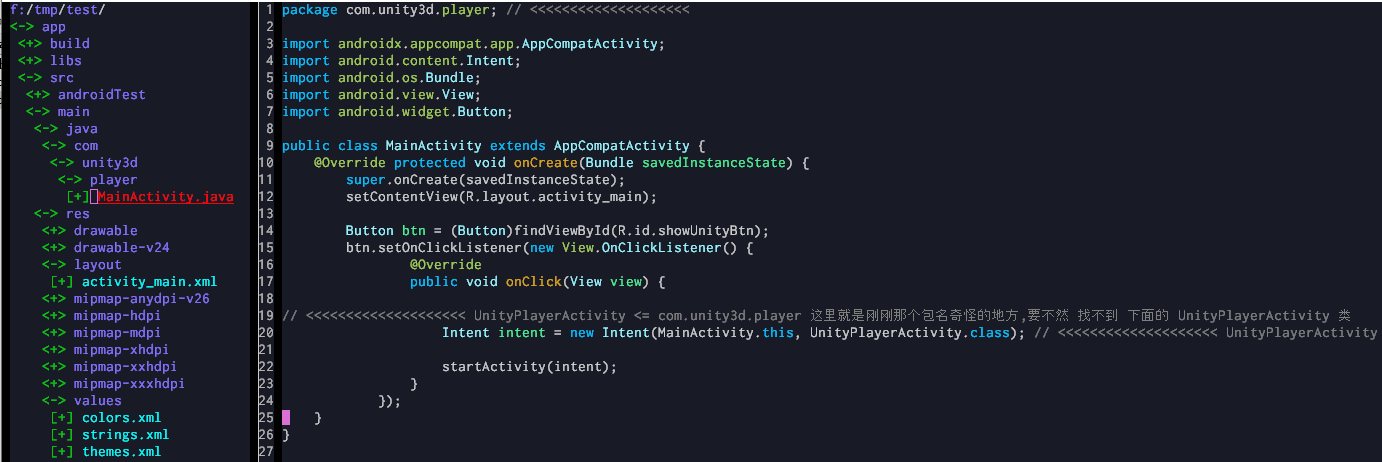
\includegraphics[width=.9\linewidth]{./pic/unityToAndroid_20221123_223852.png}
\subsection{在build.gradle中申明包裹类名称}
\label{sec-3-6}
\begin{itemize}
\item 说是现在在AndroidManifest.xml里申明包裹名称已经过时了,要在配置文件里申明,于是我在这里申明的:
\end{itemize}
\begin{minted}[fontsize=\scriptsize,linenos=false]{groovy}
android {
    namespace 'com.unity3d.player'
}
\end{minted}

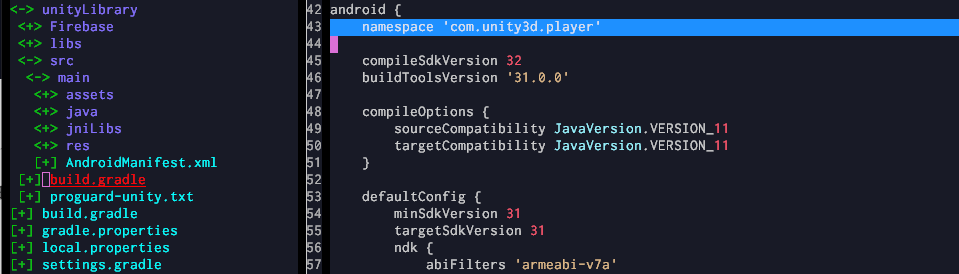
\includegraphics[width=.9\linewidth]{./pic/unityToAndroid_20221124_090438.png}

\section{启动运行}
\label{sec-4}

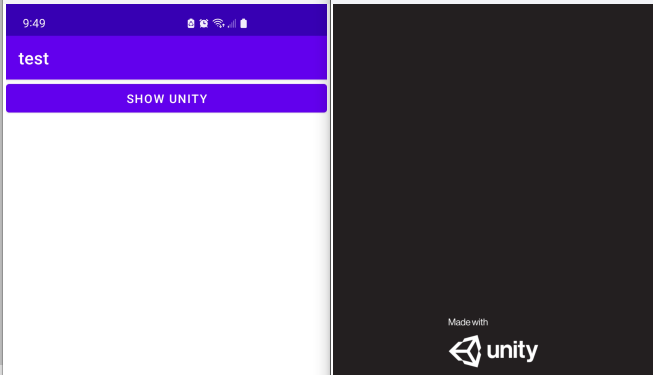
\includegraphics[width=.9\linewidth]{./pic/unityToAndroid_20221123_225517.png}

\section{那么现在就是说:安卓SDK与unity的交互与打包基本没有问题了}
\label{sec-5}
\begin{itemize}
\item 但对自己更大的挑战是:为什么unity里一个空物件挂载到热更新的过程,我打包之后在安卓手机上运行不出来,仍需要时间debug这个过程
\item 过程中遇到过,还会遇到很多不懂的问题,比如同样的某些android studio里加android:exported="true"各种标签等,如果只用unity打包,该如何实现呢?两套不同的打包机制都得弄明白.但都是这么一个学习的过程,不会被轻易挫败.
\item 相比之下,安卓SDK的实现极其简单,可以放在后面,等这些疑难杂症都解决放心了,再去写简单一点儿的
\end{itemize}
\subsection{FATAL EXCEPTION: main}
\label{sec-5-1}

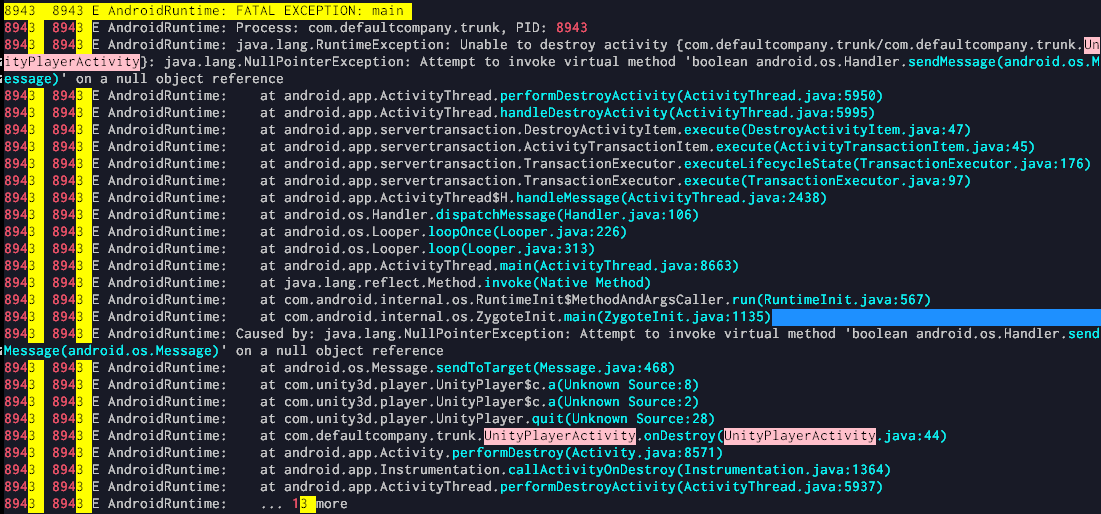
\includegraphics[width=.9\linewidth]{./pic/unityToAndroid_20221124_101807.png}
\begin{itemize}
\item 这个没有再出现了,根据这里改的:\url{https://forum.unity.com/threads/android-crashes-after-update-project-to-unity-2020-3-9f.1126979/}
\item 但是游戏的界面仍然是渲染不出来,还在找原因
\end{itemize}
\begin{minted}[fontsize=\scriptsize,linenos=false]{java}
@Override protected void onDestroy () {
    Log.d(TAG, "onDestroy() ");
    // mUnityPlayer.destroy();
    mUnityPlayer.removeAllViews();
    mUnityPlayer.quit();
    super.onDestroy();
}
\end{minted}
% Emacs 27.2 (Org mode 8.2.7c)
\end{document}